\section{実験装置}
一般的な装置の全体構成の概略を図\ref{fig:装置概略図}に示す.図\ref{fig:装置概略図}に示した装置は,ゴニオメータに X線管ならびに検出器が取り付けられ,試料を固定したままで応力を計測できる.なお,X線管を固定し,検出器や試料をゴニオメータにより走査する形式の装置もある.本実験では,X線管にはCu管を使用し,検出器には2次元位置敏感型検出器を使用して計測した.
\begin{figure}[htbp]
    \centering %中央揃え
    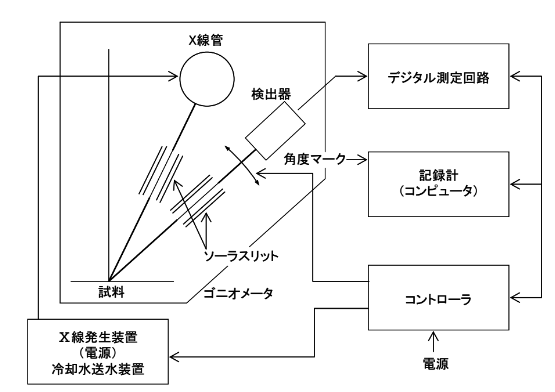
\includegraphics[width=100truemm,clip]{fig/装置概略図.png}
    \caption{Schematic of the overall configuration of a typical device.}
    \label{fig:装置概略図}
\end{figure}